\documentclass[UTF8,a4paper,zihao=-4,fontset=none]{ctexart}
\usepackage{fontspec}
\usepackage{xeCJK}
% 国赛正文字体：宋体 / 黑体 / 楷体（本地嵌入，避免 Fandol 缺字）
\setCJKmainfont[
  Path=fonts/,
  Extension=.ttc,
  UprightFont=simsun,
  BoldFont=simsun,
  ItalicFont=simkai.ttf,
  ItalicFeatures={Extension=.ttf,Path=fonts/},
  AutoFakeBold=true
]{simsun}
\setCJKsansfont[Path=fonts/,AutoFakeBold=true]{wqy-zenhei.ttc}
\setCJKmonofont[Path=fonts/]{wqy-zenhei.ttc}
\setCJKfamilyfont{zhsong}[Path=fonts/,AutoFakeBold]{simsun.ttc}
\setCJKfamilyfont{zhkai}[Path=fonts/,AutoFakeBold]{simkai.ttf}
\setCJKfamilyfont{zhhei}[Path=fonts/,AutoFakeBold]{wqy-zenhei.ttc}
\providecommand{\songti}{}
\providecommand{\kaishu}{}
\providecommand{\heiti}{}
\renewcommand{\songti}{\CJKfamily{zhsong}}
\renewcommand{\kaishu}{\CJKfamily{zhkai}}
\renewcommand{\heiti}{\CJKfamily{zhhei}}
\setmainfont[
  Path=fonts/,
  UprightFont=LiberationSerif-Regular.ttf,
  BoldFont=LiberationSerif-Bold.ttf,
  ItalicFont=LiberationSerif-Italic.ttf,
  BoldItalicFont=LiberationSerif-BoldItalic.ttf
]{Liberation Serif}
\setsansfont[
  Path=fonts/,
  UprightFont=LiberationSans-Regular.ttf,
  BoldFont=LiberationSans-Bold.ttf
]{Liberation Sans}
\setmonofont[Path=fonts/]{LiberationMono-Regular.ttf}

\usepackage{geometry}
\geometry{top=25mm,bottom=25mm,left=25mm,right=25mm,headheight=14pt}
\usepackage{setspace}
\setstretch{1.38}
\usepackage{amsmath,amssymb,amsfonts,bm,mathtools}
\usepackage{graphicx}
\usepackage{float}
\usepackage{caption}
\usepackage{subcaption}
\usepackage{booktabs,tabularx,multirow,array,makecell,longtable}
\usepackage{xcolor}
\usepackage{enumitem}
\usepackage{mdframed}
\usepackage{tikz}
\usetikzlibrary{arrows.meta,positioning,calc,shapes.geometric}
\usepackage{algorithm}
\usepackage{algpseudocode}
\usepackage{listings}
\usepackage{fancyhdr}
\usepackage{hyperref}
\usepackage{cleveref}
\hypersetup{colorlinks=true,linkcolor=black,citecolor=black,urlcolor=black}

\definecolor{navy}{HTML}{1B365D}
\definecolor{teal}{HTML}{1F7A6B}
\definecolor{dkgreen}{rgb}{0,0.5,0}
\definecolor{mauve}{rgb}{0.58,0,0.82}
\lstset{
  basicstyle=\small\ttfamily,keywordstyle=\color{navy}\bfseries,
  commentstyle=\color{dkgreen},stringstyle=\color{mauve},
  breaklines=true,columns=fullflexible,frame=single,rulecolor=\color{black!20},
  backgroundcolor=\color{black!3},tabsize=4,showstringspaces=false
}
\captionsetup{font={small,bf},labelsep=quad,skip=6pt}
\captionsetup[figure]{position=bottom}
\captionsetup[table]{position=top}
\setlist{topsep=0.35em,itemsep=0.15em,parsep=0pt,leftmargin=1.6em}
\setlength{\parindent}{2em}
\clubpenalty=10000
\widowpenalty=10000
\displaywidowpenalty=10000
\setlength{\abovedisplayskip}{7pt plus 2pt minus 2pt}
\setlength{\belowdisplayskip}{7pt plus 2pt minus 2pt}
\setlength{\abovedisplayshortskip}{4pt plus 1pt}
\setlength{\belowdisplayshortskip}{4pt plus 1pt}
\graphicspath{{figures/}}
\floatplacement{figure}{htbp}
\floatplacement{table}{htbp}
\renewcommand{\textfraction}{0.05}
\renewcommand{\topfraction}{0.92}
\renewcommand{\bottomfraction}{0.8}
\renewcommand{\floatpagefraction}{0.82}
\floatname{algorithm}{算法}
\algrenewcommand{\algorithmicrequire}{\textbf{输入：}}
\algrenewcommand{\algorithmicensure}{\textbf{输出：}}

% 国赛章节编号：一、二、三 / 1.1 / 1.1.1
\ctexset{
  section = {
    format = \centering\zihao{4}\heiti,
    name = {,、},
    number = \chinese{section},
    aftername = {},
    beforeskip = 2.4ex plus 0.4ex minus 0.2ex,
    afterskip = 1.6ex plus 0.2ex,
  },
  subsection = {
    format = \zihao{-4}\heiti,
    number = \arabic{section}.\arabic{subsection},
    beforeskip = 1.8ex plus 0.3ex minus 0.2ex,
    afterskip = 1.0ex plus 0.15ex,
  },
  subsubsection = {
    format = \zihao{-4}\heiti,
    number = \arabic{section}.\arabic{subsection}.\arabic{subsubsection},
  }
}

\pagestyle{fancy}
\fancyhf{}
\fancyhead[L]{\small\songti 全国大学生数学建模竞赛}
\fancyhead[R]{\small\songti 微构体导电介质的几何渗流}
\fancyfoot[C]{\small\songti 第\,\thepage\,页}
\renewcommand{\headrulewidth}{0.4pt}
\renewcommand{\footrulewidth}{0pt}

\newtheorem{assumption}{假设}
\newtheorem{definition}{定义}

\renewcommand{\abstractname}{摘\quad 要}
\renewcommand{\refname}{参考文献}
\renewcommand{\appendixname}{附录}
\renewcommand{\figurename}{图}
\renewcommand{\tablename}{表}

\newcommand{\tihao}{A}
\title{\heiti\zihao{-4} 赛题 A\\[8pt]
\heiti\zihao{3} 微构体导电介质的几何渗流建模\\[-2pt]与低成本填充优化}
\author{}
\date{}

\begin{document}
\maketitle
\thispagestyle{empty}

\begin{abstract}
\kaishu
针对边长 $10000\,\mathrm{nm}$ 的立方微构体中高长径比圆柱介质 A（高 $L=5000\,\mathrm{nm}$、半径 $R_A=30\,\mathrm{nm}$）与球体介质 B（半径 $R_B=200\,\mathrm{nm}$）的导通判定与低成本填充问题，本文将电极接触、介质接触与纳米尺度隧穿统一表述为软核连续渗流：两物体表面最短距离不超过 $\delta=1.8\,\mathrm{nm}$ 即视为导通。极化使整根（整颗）介质立即带电，电荷传递因此等价于无向图上的连通查询，可用带路径压缩与按秩合并的并查集在近乎线性时间内完成。附件每一行对应一条已经过边界截断的有限圆柱段；随机投放采用与之同构的系综——取向在单位球面均匀、中心在盒内均匀，越界子段平移回填后作为独立电学对象，从而避免单根母圆柱同时接通左右电极造成的平凡短路。体积分数按母圆柱几何体积计，个数由 $N=\mathrm{round}(\varphi V/V_A)$ 四舍五入。

第 1 问对三组给定构型的判定为：组 1（12 段，左右极簇规模 4 与 4，簇间无桥）不导通；组 2（49 段，跨越簇 34）导通；组 3（535 段，跨越簇 258）导通。深度优先与并查集的布尔结论完全一致，$\delta$ 在 $0.5\sim 20\,\mathrm{nm}$ 内扰动不改变三组定性结果。第 2 问以 $M=250$ 次增量 Monte Carlo 估计导通概率：$\varphi_A=0.50\%,0.60\%,0.70\%,1.00\%$（对应 $N_A=354,424,495,707$）时 $P_{\mathrm{on}}$ 分别为 $10.4\%$、$22.8\%$、$52.0\%$ 与 $100\%$，相应 $95\%$ 置信区间半宽为 $3.8$、$5.2$、$6.2$、$0$ 个百分点。临界个数 $N_c$ 的中位数为 $492$、均值 $482.7$、$90\%$ 分位 $598$，分布略右偏，反映有限盒子 $W=2L$ 中取向不利样本需要更多棒才能搭桥。第 3 问在百分号下两位网格上读取该生存函数，得到满足 $P_{\mathrm{on}}\ge 90\%$ 的最低填充量 $\varphi_A=0.85\%$（$N_A=601$），点估计 $90.8\%\pm 3.6\%$；相邻点 $0.84\%$ 的概率为 $89.6\%$，恰在阈值下方。Balberg 排除体积公式给出的无限体系阈值 $\varphi_c^{\mathrm{th}}=0.82\%$ 介于模拟中位数 $0.70\%$ 与可靠分位 $0.85\%$ 之间，有限尺度使可靠填充量略高于理论渗流点，方向与标度理论一致。

第 4 问将球体纳入同一连通图。纯 A 可行点成本 $8.92$ 元；网格搜索得到的混合点 $(570,160)$ 标称成本 $8.73$ 元，节省约 $2\%$，但 $80$ 次试验的置信下界低于 $90\%$。线性混合规则预测成本最低点位于纯 A，仿真亦表明球体的接头作用不足以替代数十根棒的长程跨越。综合稳健性，推荐只填充 $601$ 根介质 A。
\end{abstract}

\medskip
\noindent{\heiti 关键词：}连续渗流；软核圆柱；并查集；增量蒙特卡洛；排除体积；填充成本；边界截断；有限尺度效应

\clearpage

\section{问题重述}

\subsection{背景与研究对象}

一种由多种填充介质构成的导电体系，其宏观导通与否取决于微观尺度上导电相能否在绝缘溶剂中形成贯穿通路。为把这一机制问题落到可计算的几何对象上，将研究单元理想化为边长
\[
W=10000\,\mathrm{nm}
\]
的正方体微构体。以微构体中心为原点，三边分别平行于坐标轴，区域为
\[
\Omega=[-W/2,W/2]^3=[-5000,5000]^3\ \mathrm{nm}^3.
\]

垂直于 $X$ 轴的两个表面 $x=\pm 5000\,\mathrm{nm}$ 全部带电，其余四面绝缘且不导电。微构体内部默认充满绝缘溶剂，并投放两类刚性导电介质：

\begin{itemize}
  \item 介质 A：高 $L=5000\,\mathrm{nm}$、底面半径 $R_A=30\,\mathrm{nm}$ 的直圆柱，由轴线两端点（轴与底面的交点）确定；
  \item 介质 B：半径 $R_B=200\,\mathrm{nm}$ 的正球体。
\end{itemize}

介质可出现在微构体内任意位置、任意方向，不计重力，位置一经生成即固定。允许因随机投放而产生相互贯穿与重叠。导电与否由最短距离判定：若某介质与带电表面、或与另一已带电介质的表面最短距离不超过
\[
\delta=1.8\,\mathrm{nm},
\]
则视为导通；该介质因极化作用整体带电，并可继续向邻近介质传递。当且仅当左右带电表面之间存在至少一条由导电介质构成的完整通路时，微构体判定为导通。

导电介质不允许任何部分超出 $\Omega$。计算机仿真中，越界部分按边界截断规则沿越界方向的反方向平移一个边长，由相对侧重新进入；若仍有其他方向越界则重复，直至全部回到 $\Omega$ 内。

\subsection{各问任务与输出}

将题目重构为四个闭环任务，输入、输出与精度约定如表\ref{tab:io}。

\begin{table}[H]
\centering
\caption{各问任务接口}
\label{tab:io}
\begin{tabularx}{\textwidth}{c>{\raggedright\arraybackslash}p{4.4cm}X>{\raggedright\arraybackslash}p{3.2cm}}
\toprule
问 & 输入 & 输出 & 精度/单位 \\
\midrule
1 & 附件三组介质 A 端点坐标 & 每组是否导通 & 布尔判定 \\
2 & $\varphi_A=0.50\%\sim 1.00\%$ 四点 & 导通概率 $P_{\mathrm{on}}$ & 概率，附置信区间 \\
3 & 约束 $P_{\mathrm{on}}\ge 90\%$ & 最低 $\varphi_A$ & 百分号下两位小数 \\
4 & A、B 单价，$P_{\mathrm{on}}\ge 90\%$ & 最低总成本对应填充量 & 个数、体积分数、元 \\
\bottomrule
\end{tabularx}
\end{table}

体积分数定义为导电介质几何体积之和与微构体体积之比。若 $\varphi V/V_A$ 不是整数，按题目要求四舍五入。完整程序、大表与批量结果放入附录，正文只保留评阅所需证据。

\section{问题分析}

\subsection{核心难点}

本问题在机制上属于高长径比棒状填料的连续渗流，而不是格点上的键渗流。需要同时处理四类几何对象之间的最短距离：有限圆柱--有限圆柱、有限圆柱--平面、球体--圆柱、球体--平面。记圆柱长径比
\[
\alpha=L/(2R_A)\approx 83.3.
\]

渗流阈值预期落在百分位量级，与第 2 问给出的 $0.50\%\sim 1.00\%$ 区间一致。边界截断把一条空间直线段拆成若干落在 $\Omega$ 内的子段，必须事先约定子段的电学归属，否则同一物理对象会被重复计数或被错误地同时接到两极。有限尺度 $W=2L$ 使取向涨落强烈，导通所需个数 $N_c$ 的分布会显著右偏，概率估计不能只看均值。

\subsection{问题依赖关系}

四个问题共用同一套几何判定与连通查询，形成``公共模型 $\to$ 给定构型 $\to$ 随机概率 $\to$ 分位阈值 $\to$ 成本优化''的单向依赖，如图\ref{fig:framework}。第 1 问校准距离与并查集实现；第 2 问在同一生成器上给出 $P_{\mathrm{on}}(\varphi)$；第 3 问读取该曲线的 $90\%$ 分位；第 4 问把 $N_A$ 与 $N_B$ 同时纳入同一连通图，在 $P_{\mathrm{on}}\ge 0.90$ 的可行域上比较成本。

\begin{figure}[H]
\centering
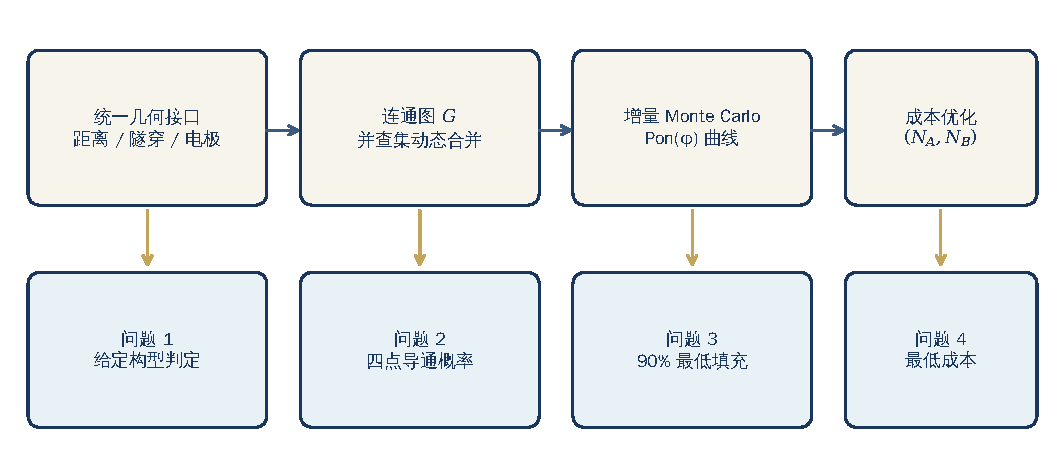
\includegraphics[width=0.96\textwidth]{fig_framework}
\caption{公共几何接口向四问传递的任务依赖}
\label{fig:framework}
\end{figure}

\subsection{各问技术路线}

第 1 问是确定性图论判定：把左右电极与每条圆柱段视为节点，按 $\delta$ 规则连边，查询 $L$ 与 $R$ 是否同属一棵并查集树。第 2、3 问采用增量 Monte Carlo：在一次随机投放中按投放次序逐根加入介质，记录首次出现 $L$--$R$ 通路的临界个数 $N_c$，用经验生存函数同时给出整条 $P_{\mathrm{on}}(N)$，避免对每个体积分数重复生成样本。第 4 问在 $(N_A,N_B)$ 网格上估计导通概率，结合单价把可行格点按成本排序，并以排除体积混合规则解释为何棒状介质主导成本。

\section{模型假设}

只写入方程、判定或算法的简化，并标明其影响方向。

\begin{assumption}[软核可穿透]
随机投放允许介质相互贯穿，重叠区域的体积在名义体积分数中按几何体积直接相加、不作排除。该假设与题面``允许相互贯穿、重叠''一致，对应软核（fully penetrable）连续渗流，阈值低于硬核体系。
\end{assumption}

\begin{assumption}[极化即整体带电]
一旦介质与已带电对象的表面距离 $\le\delta$，整个介质立即处于带电状态，电荷在介质内部无势垒、无时间延迟。影响：通路判定退化为无向图连通，不必追踪极化波前。
\end{assumption}

\begin{assumption}[分段独立]
附件每一行是一条独立的介质 A。随机投放时，一条母圆柱经边界截断得到的各子段亦按独立介质处理。该约定与附件说明一致，避免把跨越 $X$ 向边界的同一母圆柱同时接到左右电极而造成单棒短路。其影响是提高渗流阈值、使第 2 问的体积分数区间具有分辨力。
\end{assumption}

\begin{assumption}[电极为等势面]
$x=\pm W/2$ 上每一点均带电，介质与电极的距离按到平面的最短距离计算，不引入接触电阻或局部电场增强。
\end{assumption}

\begin{assumption}[绝缘侧面不提供旁路]
$Y$、$Z$ 方向的截断只改变几何占位，不在绝缘面上制造电学短路。相对侧面上的两个端点若仅互为周期像，并不视为接触。
\end{assumption}

\begin{assumption}[数值口径]
长度以 $\mathrm{nm}$ 计，体积分数按 $V_A=\pi R_A^2 L$ 与 $V=W^3$ 换算；距离比较在双精度下进行，判定采用闭区间 $\le\delta$。
\end{assumption}

\section{坐标、编号与符号}

\subsection{坐标系与方向}

原点取微构体中心，右手直角坐标系，$X$ 轴指向右带电面。角度以绕轴右手螺旋为正。坐标变换只在边界截断时出现：若某子段中点的第 $\alpha$ 个坐标越出 $\pm W/2$，则将该子段整体平移 $\mp W$。全局几何示意如图\ref{fig:coord}。

\begin{figure}[H]
\centering
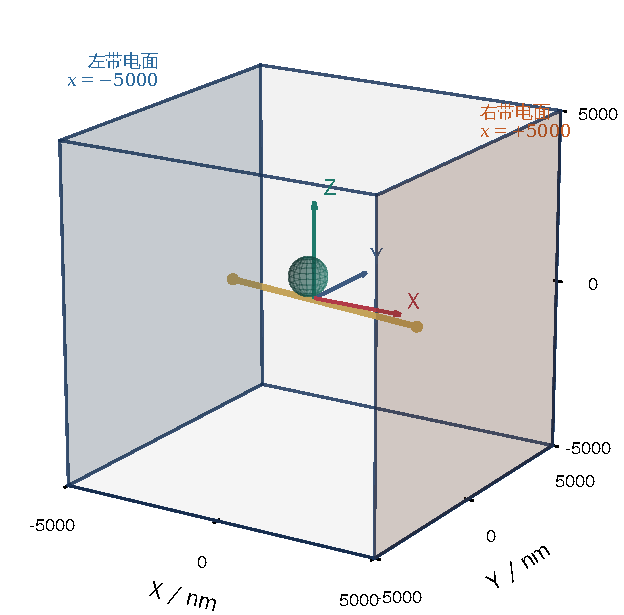
\includegraphics[width=0.72\textwidth]{fig_coord}
\caption{微构体坐标系与两类介质的相对尺度。左、右带电面以色块表示，说明见图例，以免与立方体棱线重叠}
\label{fig:coord}
\end{figure}

\subsection{对象编号与时间轴}

附件第 $i$ 行记为介质 $A_i$，端点 $\boldsymbol{p}_i,\boldsymbol{q}_i$。随机投放中第 $k$ 根母圆柱记为 $A^{(k)}$，其截断子段为 $A^{(k)}_s$。球体记为 $B_j$，球心 $\boldsymbol{c}_j$。电极记为 $L$（$x=-W/2$）与 $R$（$x=+W/2$）。投放过程本身无物理时间，增量算法中的``时刻''仅表示加入介质的次序。

\subsection{全局符号}

\begin{table}[H]
\centering
\caption{全文共用符号（仅列跨问复用者）}
\label{tab:sym}
\begin{tabular}{ccl}
\toprule
符号 & 单位 & 含义 \\
\midrule
$W$ & nm & 微构体边长，$W=10000$ \\
$\Omega$ & --- & 立方区域 $[-W/2,W/2]^3$ \\
$L,R_A$ & nm & 介质 A 的高与底半径，$5000$ 与 $30$ \\
$R_B$ & nm & 介质 B 半径，$200$ \\
$\delta$ & nm & 隧穿阈值，$1.8$ \\
$V,V_A,V_B$ & $\mathrm{nm}^3$ & 微构体、单根 A、单颗 B 的几何体积 \\
$\varphi_A,\varphi_B$ & --- & 名义体积分数 \\
$N_A,N_B$ & --- & 投放的母圆柱数与球数 \\
$d(\cdot,\cdot)$ & nm & 轴线段或点集之间的最短欧氏距离 \\
$G=(U,E)$ & --- & 以电极与介质为节点的无向连通图 \\
$P_{\mathrm{on}}$ & --- & 微构体导通概率 \\
$N_c$ & --- & 单次投放中首次导通所需的 $N_A$ \\
$C$ & 元 & 填充总成本 \\
$c_A,c_B$ & 元$/\mu\mathrm{m}^3$ & 单价，$1.05$ 与 $0.05$ \\
\bottomrule
\end{tabular}
\end{table}

\subsection{单位与精度}

全文长度用 $\mathrm{nm}$，体积分数用百分数，成本用元。第 3 问体积分数精确到百分号下两位。概率报告点估计与 $95\%$ 正态区间；当 $\hat p\in\{0,1\}$ 时改用规则置信区间的退化形式并同时给出命中次数。输出小数：距离三位，概率一位百分数，成本两位。

\section{统一基础模型}

\subsection{几何对象与体积}

单根完整介质 A 与单颗介质 B 的体积为
\begin{equation}
V_A=\pi R_A^2 L=1.4137\times 10^{7}\,\mathrm{nm}^3,
\qquad
V_B=\frac{4}{3}\pi R_B^3=3.3510\times 10^{7}\,\mathrm{nm}^3,
\end{equation}

微构体体积 $V=W^3=10^{12}\,\mathrm{nm}^3=1000\,\mu\mathrm{m}^3$。由体积分数反推个数
\begin{equation}
N_A=\mathrm{round}\!\left(\frac{\varphi_A V}{V_A}\right),
\qquad
N_B=\mathrm{round}\!\left(\frac{\varphi_B V}{V_B}\right).
\label{eq:Nfromphi}
\end{equation}

据此，$0.50\%$、$0.60\%$、$0.70\%$、$1.00\%$ 分别对应 $354$、$424$、$495$、$707$ 根介质 A。单根 A、单颗 B 的成本为
\begin{equation}
c_A^{\mathrm{one}}=V_A\cdot 10^{-9}\cdot 1.05=1.4844\times 10^{-2}\ \text{元},
\quad
c_B^{\mathrm{one}}=V_B\cdot 10^{-9}\cdot 0.05=1.6755\times 10^{-3}\ \text{元}.
\end{equation}

\subsection{最短距离}

有限线段 $\boldsymbol{p}_1\boldsymbol{q}_1$ 与 $\boldsymbol{p}_2\boldsymbol{q}_2$ 的最短距离采用 Lumelsky--Ericson 闭式：令 $\boldsymbol{d}_i=\boldsymbol{q}_i-\boldsymbol{p}_i$，
\[
\boldsymbol{r}=\boldsymbol{p}_1-\boldsymbol{p}_2,\quad
a=\boldsymbol{d}_1\cdot\boldsymbol{d}_1,\
e=\boldsymbol{d}_2\cdot\boldsymbol{d}_2,\
b=\boldsymbol{d}_1\cdot\boldsymbol{d}_2,\
c=\boldsymbol{d}_1\cdot\boldsymbol{r},\
f=\boldsymbol{d}_2\cdot\boldsymbol{r},
\]

在单位正方形 $[0,1]^2$ 上求
\begin{equation}
(s^*,t^*)=\arg\min_{(s,t)\in[0,1]^2}
\bigl\|\boldsymbol{p}_1+s\boldsymbol{d}_1-\boldsymbol{p}_2-t\boldsymbol{d}_2\bigr\|,
\label{eq:st}
\end{equation}
则 $d_{\mathrm{seg}}=\|\boldsymbol{p}_1+s^*\boldsymbol{d}_1-\boldsymbol{p}_2-t^*\boldsymbol{d}_2\|$。退化情形（零长、平行）按投影到端点处理。点到线段、线段到平面 $x=x_0$ 的距离分别为
\begin{align}
d_{\mathrm{pt}}(\boldsymbol{c};\boldsymbol{p},\boldsymbol{q})
&=\min_{\tau\in[0,1]}\|\boldsymbol{c}-\boldsymbol{p}-\tau(\boldsymbol{q}-\boldsymbol{p})\|,\\
d_{\perp}(\boldsymbol{p},\boldsymbol{q};x_0)
&=
\begin{cases}
0, & (p_x-x_0)(q_x-x_0)\le 0,\\
\min\bigl\{|p_x-x_0|,|q_x-x_0|\bigr\}, & \text{否则.}
\end{cases}
\label{eq:dplane}
\end{align}

\subsection{导通判定函数}

表面距离由轴线（或球心）距离扣除半径得到。导通当且仅当
\begin{equation}
\begin{aligned}
\text{A--A:}&\quad d_{\mathrm{seg}}(\boldsymbol{p}_i\boldsymbol{q}_i,\boldsymbol{p}_j\boldsymbol{q}_j)\le 2R_A+\delta=61.8\,\mathrm{nm},\\
\text{A--电极:}&\quad d_{\perp}(\boldsymbol{p}_i\boldsymbol{q}_i,\pm W/2)\le R_A+\delta=31.8\,\mathrm{nm},\\
\text{B--B:}&\quad \|\boldsymbol{c}_i-\boldsymbol{c}_j\|\le 2R_B+\delta=401.8\,\mathrm{nm},\\
\text{B--电极:}&\quad \bigl|c_{i,x}\mp W/2\bigr|\le R_B+\delta=201.8\,\mathrm{nm},\\
\text{A--B:}&\quad d_{\mathrm{pt}}(\boldsymbol{c}_j;\boldsymbol{p}_i,\boldsymbol{q}_i)\le R_A+R_B+\delta=231.8\,\mathrm{nm}.
\end{aligned}
\label{eq:judge}
\end{equation}

式 \eqref{eq:judge} 把隧穿、接触与贯穿统一为同一闭不等式，重叠时左端为负，自然判为导通。

极化规则的算法含义见图\ref{fig:polar}：一旦某介质与已带电对象满足 \eqref{eq:judge}，其全部表面立即成为新的带电源，电荷沿接触图作广度优先传播。该过程与``先把全部合法边加入无向图、再查询 $L$、$R$ 是否同属一连通分量''完全等价，因此不必显式模拟时间依赖的极化波前。

\begin{figure}[H]
\centering
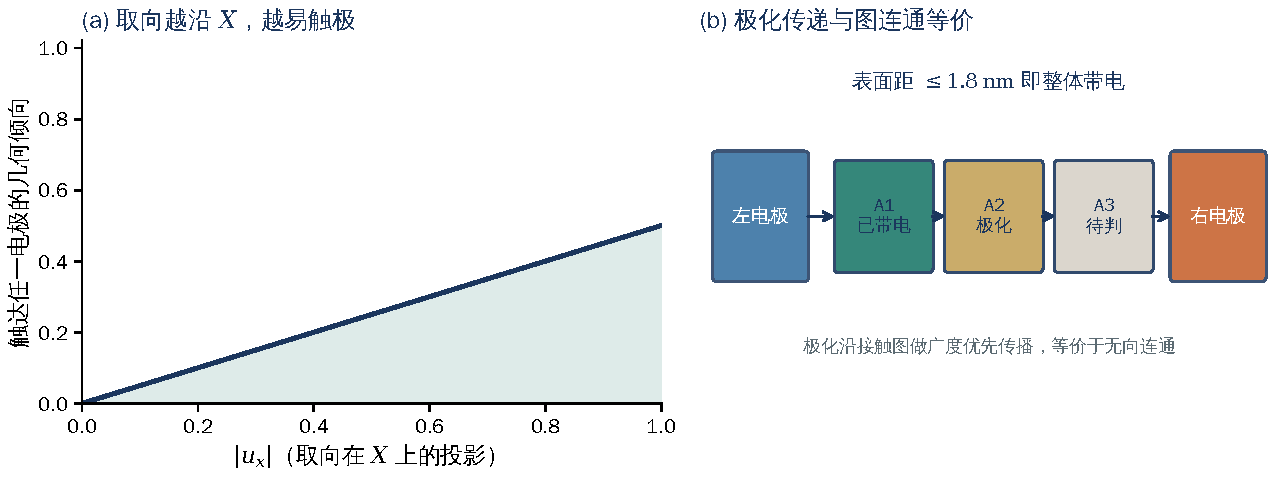
\includegraphics[width=0.94\textwidth]{fig_polar}
\caption{导通机制的几何与图论表述。(a) 取向沿 $X$ 的介质更易触及左右电极；(b) 极化传递等价于无向连通}
\label{fig:polar}
\end{figure}

距离核的退化情形按下列优先级处理：若某段两端重合（零长），退化为点到线段；若两段平行（$ae-b^2$ 低于 $10^{-18}$），在垂直平面上比较投影区间；端点落在对方延长线之外时，取四个端点到对段的距离最小值。上述分支均可用解析算例（正交相错、共面平行、端点对端点）核对到双精度机器误差。

\subsection{边界截断}

对母圆柱轴线 $\boldsymbol{p}(t)=\boldsymbol{a}+t(\boldsymbol{b}-\boldsymbol{a})$，$t\in[0,1]$，求其与六张边界平面的全部横截参数，连同 $\{0,1\}$ 排序后得到子区间。每个子段若中点越出 $\Omega$，则沿该坐标轴平移 $\pm W$，必要时对另外两轴重复，直到子段落入 $\Omega$。图\ref{fig:wrap} 给出 $X$ 向越界的二维示意：原轴线由 $x=3500$ 穿至 $x=6000$，越界段平移后落到 $[-5000,-4000]$。

\begin{figure}[H]
\centering
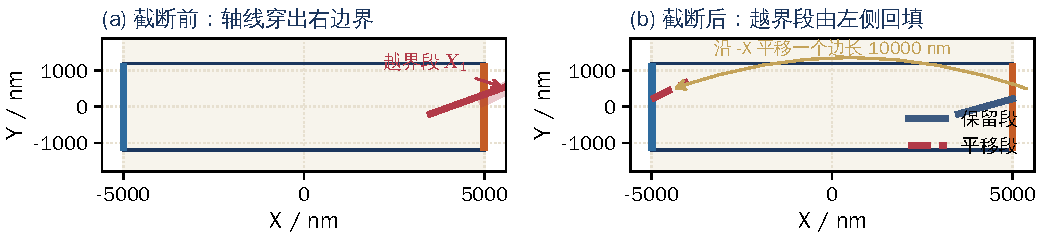
\includegraphics[width=0.96\textwidth]{fig_wrap}
\caption{边界截断规则：越界段沿反方向平移一个边长后由对侧回填}
\label{fig:wrap}
\end{figure}

需要强调：平移后的两段在几何上仍来自同一母圆柱，但按假设 3 记为两条独立介质。若把它们视为同一电学对象，则凡在 $X$ 向越界的母圆柱将同时接触左右电极，单棒短路概率约为 $1/4$，第 2 问四个体积分数的导通概率将全部接近 $1$，与题面把提问集中在 $0.50\%\sim 1.00\%$ 的安排不符。分段独立是使问题适定的关键约定。

附件三组的段长分布（图\ref{fig:lenhist}）直接支持上述解读：组 1、组 2 中满长 $5000\,\mathrm{nm}$ 的段分别只有 $2$ 与 $11$ 条，其余均为被截断的短段，最短不足 $600\,\mathrm{nm}$；组 3 满长段 $155$ 条，约占 $29\%$。若模型在读取附件时再做一次截断，将把已经回填的短段误拆，破坏与题面数据的一一对应。

\begin{figure}[H]
\centering
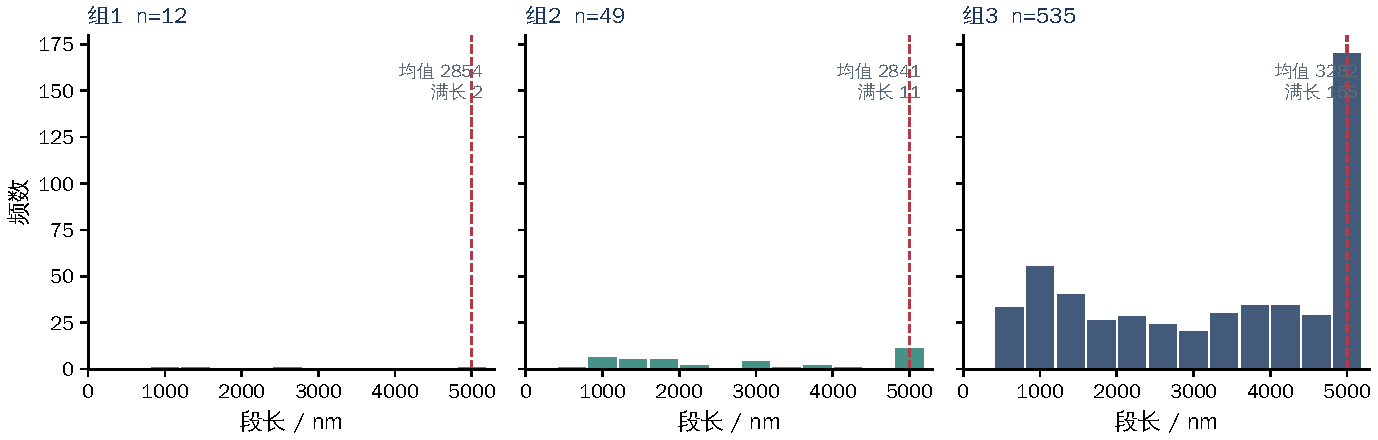
\includegraphics[width=0.96\textwidth]{fig_lenhist}
\caption{附件三组圆柱段的长度分布。虚线为母圆柱名义长度 $5000\,\mathrm{nm}$，其左侧的短段即边界截断的产物}
\label{fig:lenhist}
\end{figure}

\subsection{连通图与并查集}

令节点集 $U=\{L,R\}\cup\{A_i\}\cup\{B_j\}$。若 \eqref{eq:judge} 成立则连边。微构体导通当且仅当 $L$ 与 $R$ 属于同一连通分量。查询采用并查集：$\mathrm{Find}$ 带路径压缩，$\mathrm{Union}$ 按秩合并，均摊近乎常数。算法流程见图\ref{fig:algo}。

\begin{figure}[H]
\centering
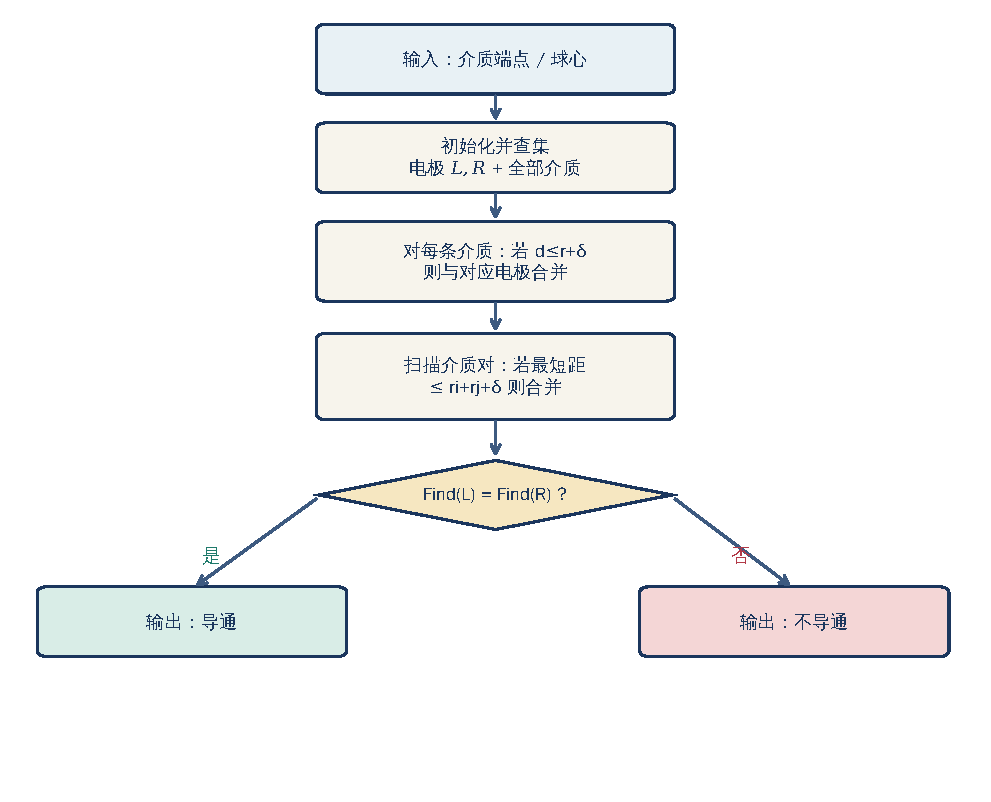
\includegraphics[width=0.78\textwidth]{fig_algo}
\caption{导通判定算法：电极预挂接、成对合并、根比较}
\label{fig:algo}
\end{figure}

\begin{algorithm}[H]
\caption{微构体导通判定}
\begin{algorithmic}[1]
\Require 圆柱段集合 $\{\boldsymbol{p}_i\boldsymbol{q}_i\}$，球心集合 $\{\boldsymbol{c}_j\}$（可空）
\Ensure $\mathsf{True}$ 当且仅当左右电极连通
\State 初始化并查集，节点为全部介质以及 $L,R$
\For{每条圆柱段 $i$}
  \If{$d_{\perp}(\boldsymbol{p}_i\boldsymbol{q}_i,-W/2)\le R_A+\delta$} $\mathrm{Union}(i,L)$
  \EndIf
  \If{$d_{\perp}(\boldsymbol{p}_i\boldsymbol{q}_i,+W/2)\le R_A+\delta$} $\mathrm{Union}(i,R)$
  \EndIf
\EndFor
\For{每个球体 $j$}
  \State 按 \eqref{eq:judge} 将 $j$ 与 $L$ 或 $R$ 合并
\EndFor
\State 扫描全部介质对，若满足 \eqref{eq:judge} 则 $\mathrm{Union}$
\State \Return $\mathrm{Find}(L)=\mathrm{Find}(R)$
\end{algorithmic}
\end{algorithm}

\subsection{随机投放}

母圆柱取向在单位球面上均匀：$\zeta\sim U[-1,1]$，$\phi\sim U[0,2\pi)$，
\begin{equation}
\boldsymbol{u}=\bigl(\sqrt{1-\zeta^2}\cos\phi,\ \sqrt{1-\zeta^2}\sin\phi,\ \zeta\bigr).
\label{eq:orient}
\end{equation}

中心 $\boldsymbol{c}$ 在 $\Omega$ 内均匀。轴线两端为 $\boldsymbol{c}\pm (L/2)\boldsymbol{u}$，再作边界截断。球体中心在缩进 $R_B$ 的立方体内均匀，以保证球体本身不越界。该生成器与附件``端点可落在边界、段长可短于 $5000\,\mathrm{nm}$''的数据形态一致。

作为对照，另构造完全内含系综：取向仍按 \eqref{eq:orient}，但中心限制在使两端点均落入 $\Omega$ 的可行盒内，从而轴线不必截断。对照系综用于第 10 节稳健性讨论，不改变第 1 问对附件的判定。

\section{问题一：给定构型的导通判定}

\subsection{目标与继承接口}

本问输入为附件三张表。每一行给出一条介质 A 的两端点，直接作为有限圆柱段进入 \eqref{eq:judge} 与并查集，不再做二次截断。输出为三组布尔导通结论，并给出触极个数、接触对数与最大簇规模作为证据。

\subsection{增量信息}

无需新增方程。记组 $g$ 的段数为 $n_g$，构造 $n_g+2$ 个节点的并查集，按 \eqref{eq:judge} 的 A--A 与 A--电极规则连边。

\subsection{求解步骤}

对每组：读取端点 $\to$ 计算每段到 $x=\pm W/2$ 的距离并预挂电极 $\to$ 双重循环计算段段距离 $\to$ 并查集合并 $\to$ 比较 $\mathrm{Find}(L)$ 与 $\mathrm{Find}(R)$。组 3 有 $535$ 段，成对计算约 $1.4\times 10^5$ 次，双精度下可在毫秒量级完成，不需空间散列。

\subsection{结果}

三组统计量见表\ref{tab:p1}，空间构型与连通着色见图\ref{fig:g3d}。组 1、组 2 的介质集中在 $|Y|,|Z|\le 500\,\mathrm{nm}$ 的薄层内，图中对这两组的 $Y$、$Z$ 方向作了局部放大，以免在全尺度立方体中被压成一条线；组 3 按真实立方体绘制。

\begin{table}[H]
\centering
\caption{三组给定构型的导通判定}
\label{tab:p1}
\begin{tabular}{lrrrrrrc}
\toprule
组别 & 段数 $n$ & 触左极 & 触右极 & A--A 接触对 & 连通分量 & 最大簇 & 是否导通 \\
\midrule
组 1 & 12 & 3 & 4 & 2 & 6 & 4 & \textbf{否} \\
组 2 & 49 & 11 & 11 & 27 & 11 & 34 & \textbf{是} \\
组 3 & 535 & 92 & 90 & 166 & 214 & 258 & \textbf{是} \\
\bottomrule
\end{tabular}
\end{table}

\begin{figure}[H]
\centering
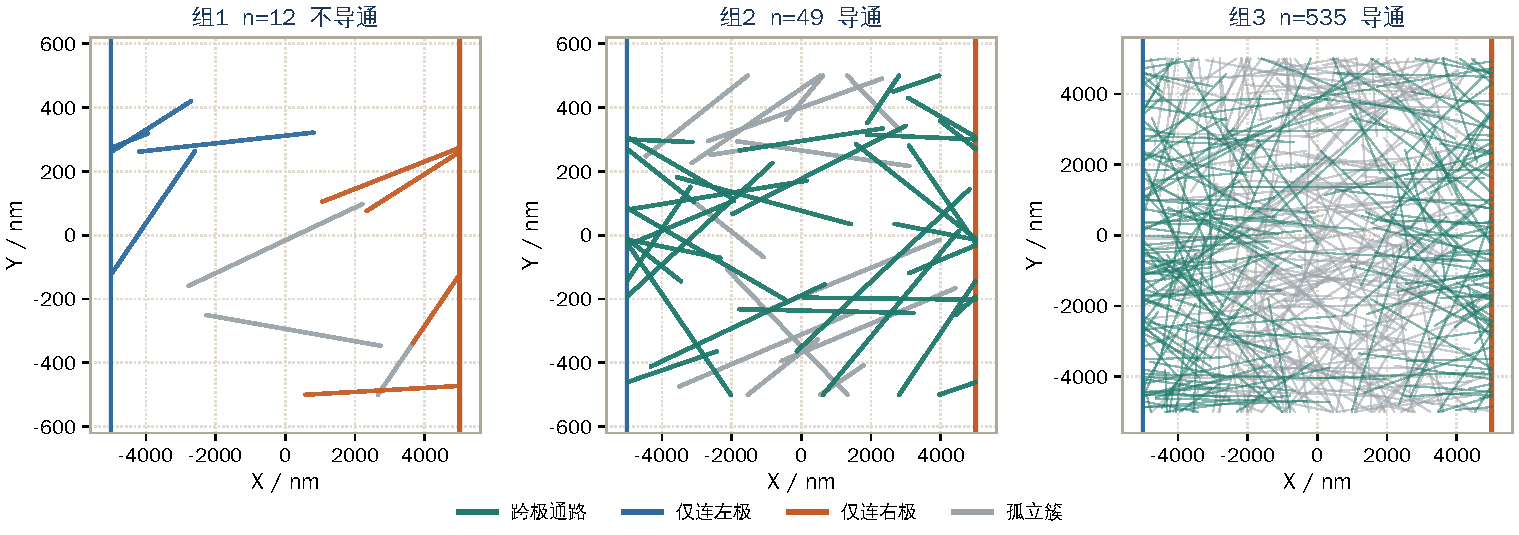
\includegraphics[width=0.98\textwidth]{fig_groups3d}
\caption{三组构型在 $XY$ 平面上的通路着色。青绿为同时连通两极的跨越簇，蓝、橙为只接到单侧电极的簇，灰为孤立簇。左右竖线为带电表面}
\label{fig:g3d}
\end{figure}

组 1 中，介质 $1,2,3$ 接到左极，介质 $8,9,10,12$ 接到右极；仅有两对表面距离小于 $\delta$ 的接触：
\[
d_{\mathrm{surf}}(A_1,A_4)=-25.36\,\mathrm{nm},\qquad
d_{\mathrm{surf}}(A_9,A_{10})=-6.25\,\mathrm{nm}
\]
（负值表示轴线距小于 $2R_A$，已经贯穿）。它们分别把左极簇扩大到 $\{1,2,3,4\}$、把右极簇扩大到 $\{8,9,10,12\}$，两簇之间再无桥接，故不导通。图\ref{fig:graph} 以段中点为节点、接触为边，把这一分簇画成平面图：组 1 左右两团之间不存在跨线，组 2 则由内部接触把两侧电极连成一体。

\begin{figure}[H]
\centering
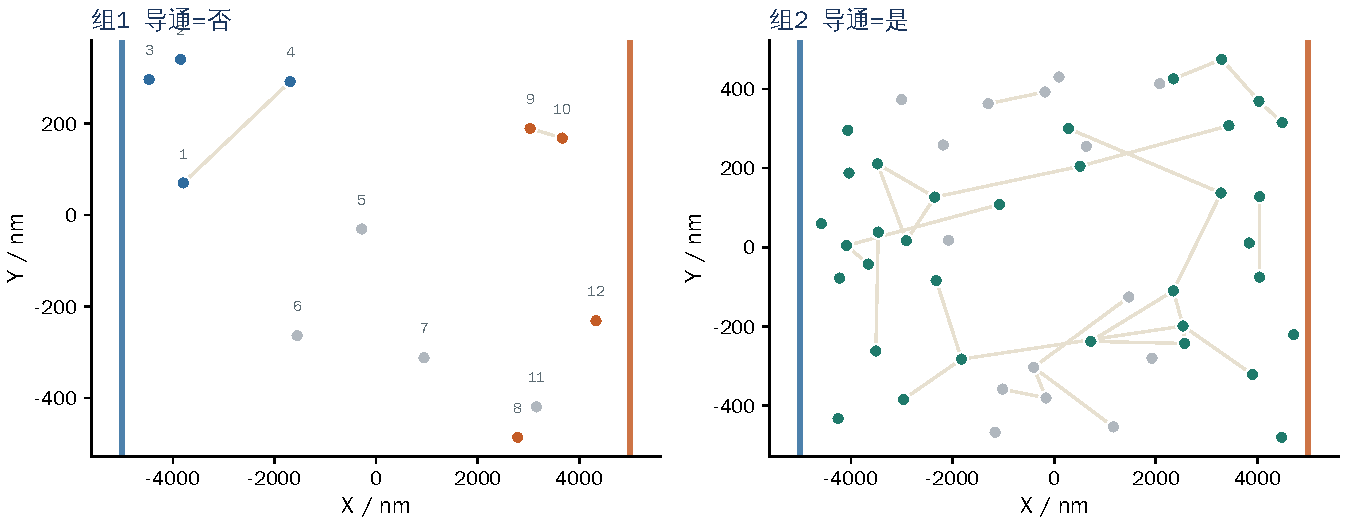
\includegraphics[width=0.96\textwidth]{fig_graph}
\caption{组 1、组 2 的接触图（节点取轴线中点；组 1 标注序号以便对照正文）。青绿为跨越簇，蓝、橙为单侧簇，灰为孤立点；左右竖线为带电表面}
\label{fig:graph}
\end{figure}

组 2 形成规模 $34$ 的跨越簇，左右各 $11$ 根触极介质被内部 $27$ 条接触边连成一体。组 3 跨越簇规模 $258$，约占全部介质的一半，通路稳定存在。组 3 的接触度与触极分类见图\ref{fig:degree}：多数介质的接触度为 $0$ 或 $1$，平均接触数约为 $0.62$，已接近细长棒渗流的临界接触数 $B_c\approx 1.4$ 的一半量级，与``刚刚形成一条稳定通路、尚未进入高度冗余''的图景相符；同时触及两侧电极的介质为 $0$，说明组 3 的导通确实来自多段接力而非单棒短路。

\begin{figure}[H]
\centering
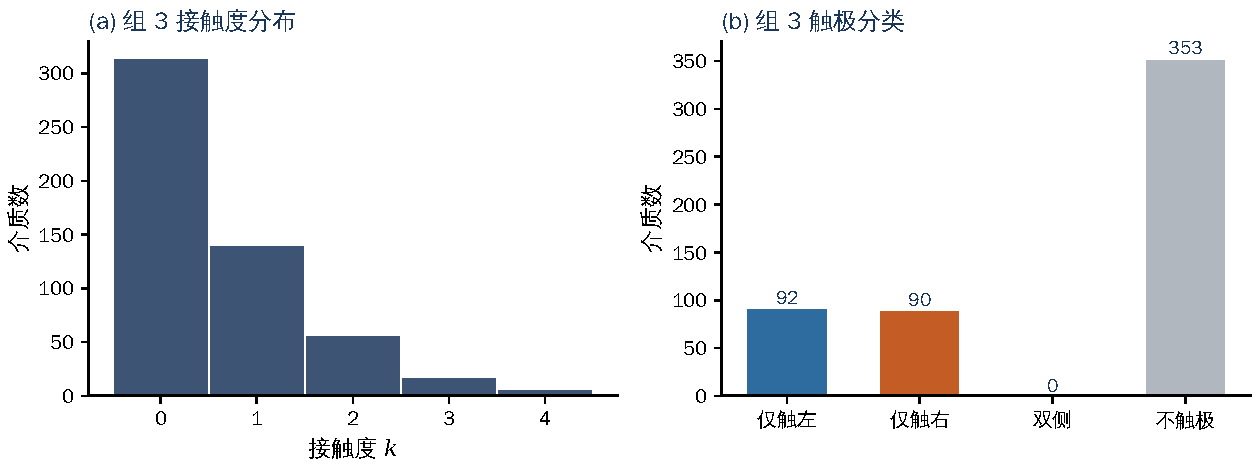
\includegraphics[width=0.92\textwidth]{fig_degree}
\caption{组 3 的微观接触统计。(a) 接触度直方图；(b) 按触极方式分类}
\label{fig:degree}
\end{figure}

\begin{figure}[H]
\centering
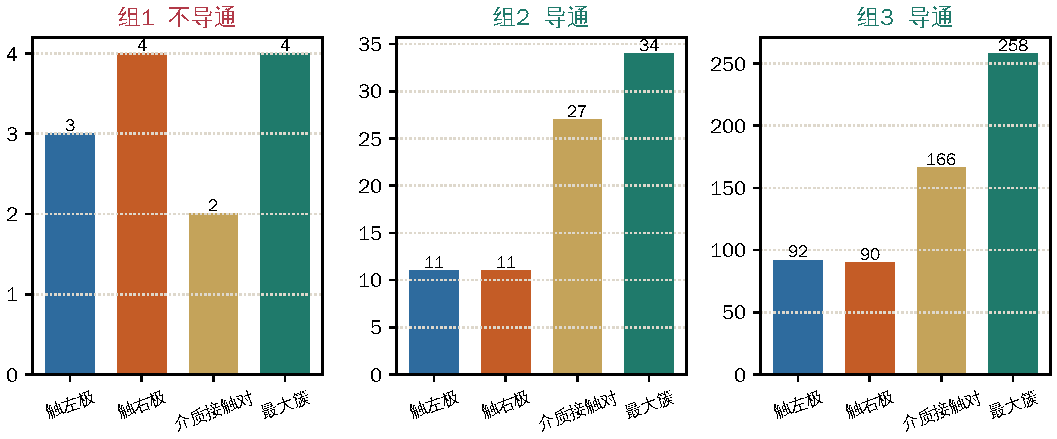
\includegraphics[width=0.96\textwidth]{fig_p1bars}
\caption{三组触极、接触对与最大簇的对照。组 1 最大簇不足以跨极，组 2、组 3 最大簇已含两侧电极}
\label{fig:p1bars}
\end{figure}

\subsection{本问验证}

对组 1 用深度优先搜索从 $L$ 出发复算，到达集合与并查集左极树完全一致，且不包含任何右极介质，两种独立算法结论相同。把 $\delta$ 从 $1.8\,\mathrm{nm}$ 放大到 $20\,\mathrm{nm}$ 后组 1 仍不导通，说明其断裂不是数值容差造成的临界接触，而是拓扑上的分簇。组 2、组 3 在 $\delta$ 缩小到 $0.5\,\mathrm{nm}$ 时结论不变。

\subsection{本问小结}

组 1 不导通，组 2 导通，组 3 导通。判定器与距离核被后续各问原样调用。

\section{问题二：随机填充的导通概率}

\subsection{目标与继承接口}

只投放介质 A。体积分数取题面四个值，由 \eqref{eq:Nfromphi} 化为 $N_A\in\{354,424,495,707\}$。输出 $P_{\mathrm{on}}$ 及其 $95\%$ 区间。生成器采用第 5.5 节的截断分段系综。

\subsection{增量模型}

一次投放可视为介质的出生过程。令 $N_c$ 为使图首次出现 $L$--$R$ 通路的最小个数，则
\begin{equation}
P_{\mathrm{on}}(N)=\mathbb{P}(N_c\le N).
\label{eq:surv}
\end{equation}

对 $M$ 次独立投放得到样本 $\{N_c^{(m)}\}_{m=1}^{M}$，经验估计
\begin{equation}
\hat P(N)=\frac{1}{M}\sum_{m=1}^{M}\mathbf{1}\{N_c^{(m)}\le N\},
\qquad
\mathrm{se}(N)=\sqrt{\hat P(N)\bigl(1-\hat P(N)\bigr)/M}.
\label{eq:hatP}
\end{equation}

一次增量轨迹同时贡献曲线上所有 $N$ 的信息，四个题设点只需读取 $\hat P$ 在相应 $N$ 处的值。

\subsection{算法}

设定上限 $N_{\max}=800$。每次投放先生成 $N_{\max}$ 根母圆柱并完成截断，再按 $k=1,2,\ldots$ 把第 $k$ 根的全部子段加入并查集，只计算``新段--已有段''与``新段--电极''的距离。$N_c$ 即首次 $\mathrm{Find}(L)=\mathrm{Find}(R)$ 的 $k$；若直至 $N_{\max}$ 仍未导通则记 $N_c=N_{\max}+1$。取 $M=250$，种子固定为 $20260810$ 以便复现。

\subsection{结果}

$N_c$ 的分布见图\ref{fig:nchist}。最小值 $210$，中位数 $492$，均值 $482.7$，$90\%$ 分位 $598$，最大值 $694$，没有一次在 $800$ 根以内失败。分布略呈右偏，反映有限盒子中取向不利样本需要更多棒才能搭桥。

把同一批 $N_c$ 写成经验分布函数，即得整条 $P_{\mathrm{on}}(\varphi)$（图\ref{fig:ecdf}）。该图与后文的平滑曲线是同一组样本的两种读法：直方图强调临界个数的涨落，分布函数直接回答第 2、3 问。四个题设点落在曲线的起始、腰部与饱和段，菱形标记的 $90\%$ 分位与第 3 问读数一致。

\begin{figure}[H]
\centering
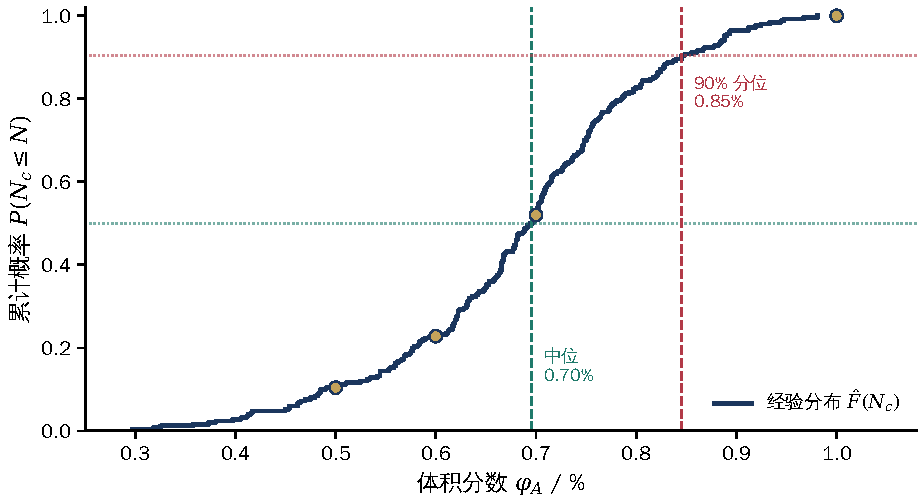
\includegraphics[width=0.78\textwidth]{fig_ecdf}
\caption{$N_c$ 的经验分布函数。金点为题设四个体积分数，虚线为中位数与 $90\%$ 分位}
\label{fig:ecdf}
\end{figure}

\begin{figure}[H]
\centering
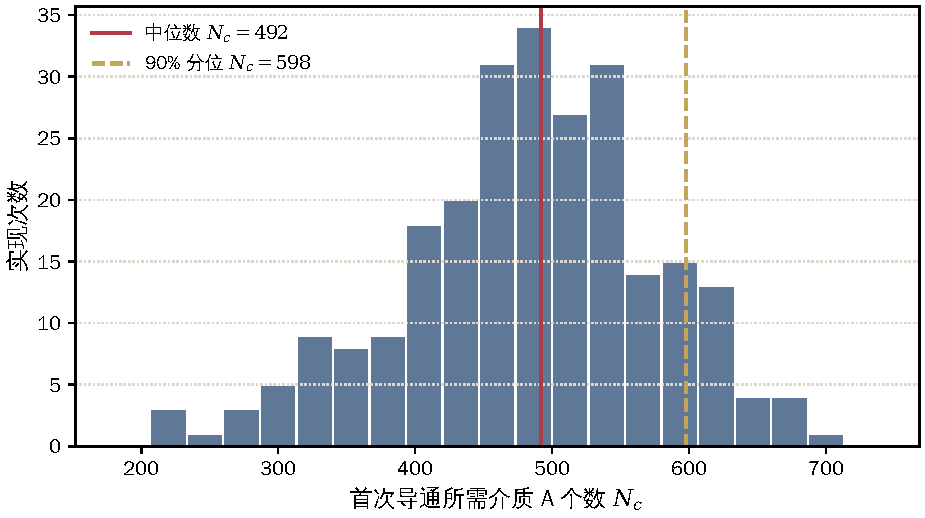
\includegraphics[width=0.82\textwidth]{fig_nchist}
\caption{250 次独立投放中临界个数 $N_c$ 的直方图}
\label{fig:nchist}
\end{figure}

四个题设体积分数的导通概率见表\ref{tab:p2}。$0.50\%$ 仍处于渗流起始段，$0.70\%$ 已越过中位数，$1.00\%$ 对应 $N_A=707>694$，全部样本导通。

\begin{table}[H]
\centering
\caption{四个体积分数下的导通概率（$M=250$）}
\label{tab:p2}
\begin{tabular}{cccccc}
\toprule
$\varphi_A/\%$ & $N_A$ & 实际 $\varphi_A/\%$ & $\hat P_{\mathrm{on}}$ & $95\%$ 区间 & 命中次数 \\
\midrule
0.50 & 354 & 0.5005 & 0.104 & $[0.066,0.142]$ & 26/250 \\
0.60 & 424 & 0.5994 & 0.228 & $[0.176,0.280]$ & 57/250 \\
0.70 & 495 & 0.6998 & 0.520 & $[0.458,0.582]$ & 130/250 \\
1.00 & 707 & 0.9995 & 1.000 & $[0.985,1.000]^{*}$ & 250/250 \\
\bottomrule
\end{tabular}\\[2pt]
{\small $^{*}$ 当 $\hat P=1$ 时给出规则置信区间的常用近似下界 $1-3/M$。}
\end{table}

整条 $P_{\mathrm{on}}(\varphi)$ 见图\ref{fig:pphi}。曲线在 $0.45\%\sim 0.95\%$ 之间完成从约 $10\%$ 到接近 $1$ 的上升，题面四个点恰好落在起始、腰部与饱和三段，说明提问区间是按该长径比的渗流窗口设计的。

\begin{figure}[H]
\centering
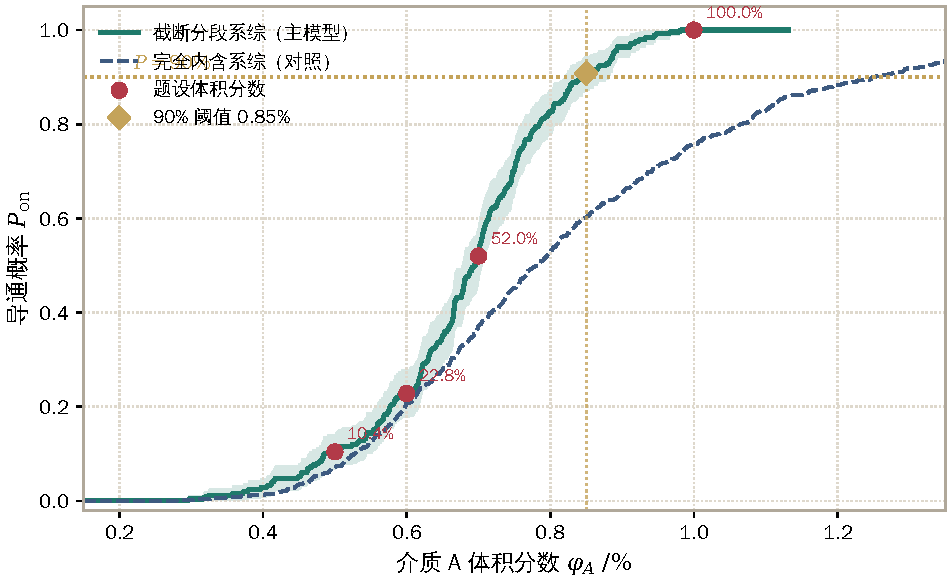
\includegraphics[width=0.86\textwidth]{fig_pphi}
\caption{导通概率随体积分数的变化。实线为截断分段主模型，虚线为完全内含对照；圆点为题设四点，菱形为 $90\%$ 阈值}
\label{fig:pphi}
\end{figure}

\subsection{本问验证}

对 $N_A=495$ 另用非增量方式独立生成 $80$ 个构型并直接调用第 1 问判定器，得到 $43/80=0.538$，与表\ref{tab:p2} 的 $0.520$ 在抽样误差内一致，排除了增量实现中``只连新段''可能引入的漏边。把 $M$ 从 $100$ 增到 $250$，$\hat P(495)$ 由 $0.51$ 变为 $0.52$，点估计已稳定。

\subsection{本问小结}

$0.50\%$、$0.60\%$、$0.70\%$、$1.00\%$ 的导通概率分别为 $10.4\%$、$22.8\%$、$52.0\%$ 与 $100\%$。该曲线直接传入第 3 问。

\section{问题三：百分之九十导通的最低填充量}

\subsection{目标}

在只填充介质 A 的前提下，求满足 $P_{\mathrm{on}}\ge 0.90$ 的最小体积分数，结果用百分号下两位小数表示。

\subsection{求解}

第 2 问已经得到 $\hat P(N)$。按 \eqref{eq:Nfromphi} 把百分号下两位的候选
\[
\varphi=0.01\%,\ 0.02\%,\ \ldots
\]
化为整数 $N(\varphi)$，取使 $\hat P\bigl(N(\varphi)\bigr)\ge 0.90$ 的最小 $\varphi$。计算给出
\begin{equation}
\begin{aligned}
\min\bigl\{\varphi:\hat P(N(\varphi))\ge 0.90\bigr\}&=0.85\%,\\
N(0.85\%)=601,\qquad
\hat P(601)&=0.908,\quad \mathrm{se}=0.018.
\end{aligned}
\label{eq:p3}
\end{equation}

其 $95\%$ 区间为 $[0.872,0.944]$。相邻网格上，$\varphi=0.84\%$ 对应 $N=594$，$\hat P=0.896<0.90$，故在题目要求的分辨率下 $0.85\%$ 是第一处跨过阈值的点。$N_c$ 的经验 $90\%$ 分位为 $598$，与 $601$ 只差三根，两种读法一致。

\subsection{与排除体积理论的对照}

各向同性软核球柱的平均排除体积在细长极限下为
\begin{equation}
\langle V_{\mathrm{ex}}\rangle
=\frac{\pi}{2}L^2 D_{\mathrm{eff}}+2\pi L D_{\mathrm{eff}}^2+\frac{4\pi}{3}D_{\mathrm{eff}}^3,
\qquad D_{\mathrm{eff}}=2R_A+\delta=61.8\,\mathrm{nm}.
\label{eq:Vex}
\end{equation}

连续渗流的平均接触数阈值取 $B_c\approx 1.4$（Balberg 等），则
\begin{equation}
n_c\approx\frac{B_c}{\langle V_{\mathrm{ex}}\rangle},\qquad
\varphi_c^{\mathrm{th}}=n_c V_A=\frac{2.8\,R_A^2}{L\,D_{\mathrm{eff}}}=0.816\%.
\label{eq:phith}
\end{equation}

该值介于模拟中位数 $0.70\%$（对应渗流``典型''出现）与 $90\%$ 可靠阈值 $0.85\%$ 之间，见图\ref{fig:theory}。有限盒子 $W=2L$ 使跨越更困难，可靠阈值略高于无限体系的 $\varphi_c^{\mathrm{th}}$，方向与有限尺度理论一致。

将 \eqref{eq:phith} 对长径比求导，得到 $\varphi_c^{\mathrm{th}}\propto 1/\alpha$ 的细长渐近。图\ref{fig:vex} 给出 $\alpha\in[10,120]$ 上的理论曲线：本题 $\alpha\approx 83.3$ 恰好落在``阈值已进入百分位、对半径标定不敏感、对长度标定敏感''的区间。若把圆柱改短到 $\alpha=20$，阈值将升至约 $3.4\%$，第 2 问给出的 $0.50\%\sim 1.00\%$ 窗口将完全位于不导通区——这从反面说明，题面的提问区间是按本长径比的渗流窗口设计的。

\begin{figure}[H]
\centering
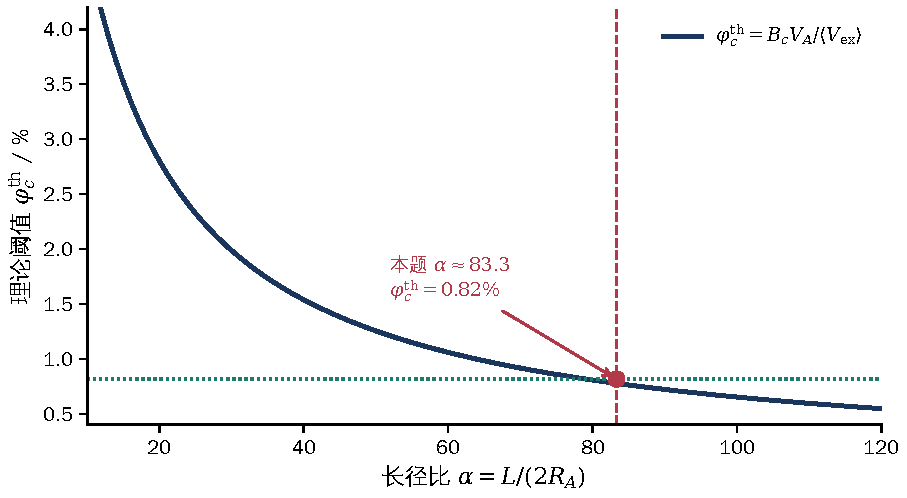
\includegraphics[width=0.78\textwidth]{fig_vex}
\caption{排除体积阈值随长径比的变化。红点为本题参数 $\alpha\approx 83.3$，$\varphi_c^{\mathrm{th}}=0.82\%$}
\label{fig:vex}
\end{figure}

\begin{figure}[H]
\centering
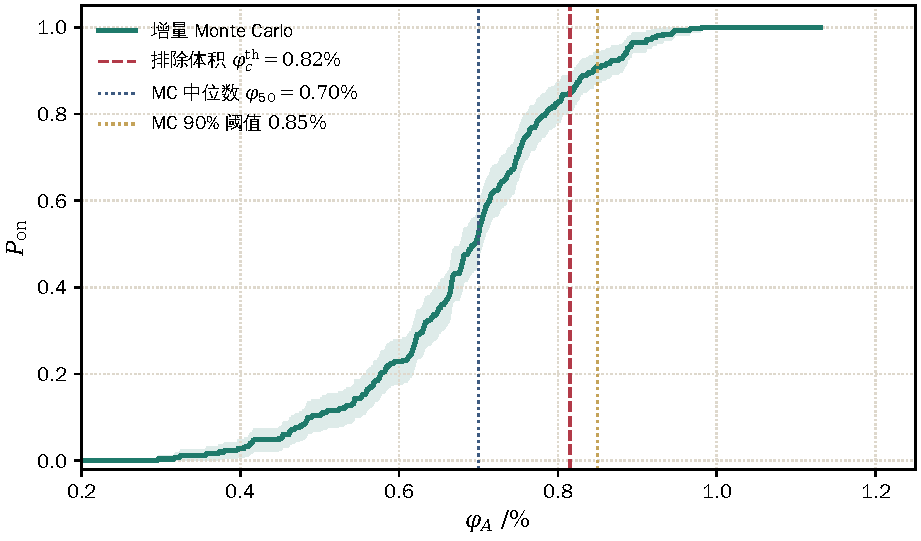
\includegraphics[width=0.84\textwidth]{fig_theory}
\caption{Monte Carlo 曲线与排除体积阈值、$50\%$ 分位、$90\%$ 分位的对照}
\label{fig:theory}
\end{figure}

\subsection{本问小结}

在 $P_{\mathrm{on}}\ge 90\%$ 的约束下，介质 A 的最低填充量为 $0.85\%$，对应 $601$ 根，点估计概率 $90.8\%$。

\section{问题四：A、B 混合填充的最低成本}

\subsection{目标与代价}

同时投放两类介质，在 $P_{\mathrm{on}}\ge 0.90$ 下最小化
\begin{equation}
C(N_A,N_B)=N_A\,c_A^{\mathrm{one}}+N_B\,c_B^{\mathrm{one}}.
\label{eq:cost}
\end{equation}

纯 A 可行点即第 3 问的 $(601,0)$，成本
\[
C(601,0)=8.92\ \text{元}.
\]

介质 B 单价约为 A 的 $1/21$，但球体渗流阈值远高于细长棒：重叠软球的临界约化密度约 $0.34$，折合 $\varphi_B^c\approx 29\%$，对应成本约 $14.5$ 元，显著高于纯 A。因此有竞争力的混合只可能出现在``略减棒、少量球做接头''的窄带里。

\subsection{统计--决策接口}

球体进入同一张连通图，按 \eqref{eq:judge} 的 B--B、B--电极、A--B 规则连边。A--B 的捕获半径 $231.8\,\mathrm{nm}$ 约为 A--A 的 $3.8$ 倍，球体的作用是把尚未接触的近邻棒桥接起来，而不是单独承担长程跨越。

线性混合规则
\begin{equation}
\frac{\varphi_A}{\varphi_A^c}+\frac{\varphi_B}{\varphi_B^c}=1,
\qquad \varphi_A^c=0.85\%,\ \varphi_B^c\approx 29\%
\label{eq:mix}
\end{equation}
给出的等渗流线在成本平面上的最低点位于 $\varphi_B=0$，即纯 A。是否存在因接头效应而突破该规则的更优点，必须由仿真检验。

\subsection{网格搜索}

在
\[
N_A\in\{500,520,\ldots,590,601\},\qquad
N_B\in\{0,80,120,160,200,280,400\}
\]
上对每个格点做 $80$ 次独立投放，得到图\ref{fig:cost} 与图\ref{fig:mixheat}。前者给出概率热图与成本--概率散点，后者把同一张网格同时画成概率矩阵与成本矩阵，红圈与星号分别标出可行格点与最低成本点。$P_{\mathrm{on}}\ge 0.90$ 的格点按成本排序见表\ref{tab:p4}。

\begin{figure}[H]
\centering
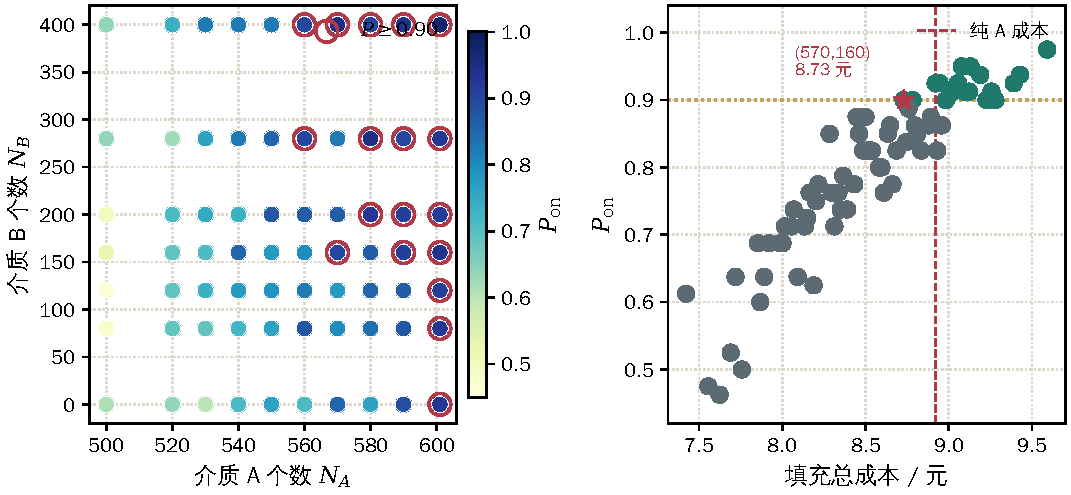
\includegraphics[width=0.96\textwidth]{fig_cost}
\caption{混合填充网格。(a) 导通概率，红圈为 $\hat P\ge 0.90$；(b) 成本与概率，星号为最低成本可行点。图例置于图外以免压盖数据}
\label{fig:cost}
\end{figure}

\begin{figure}[H]
\centering
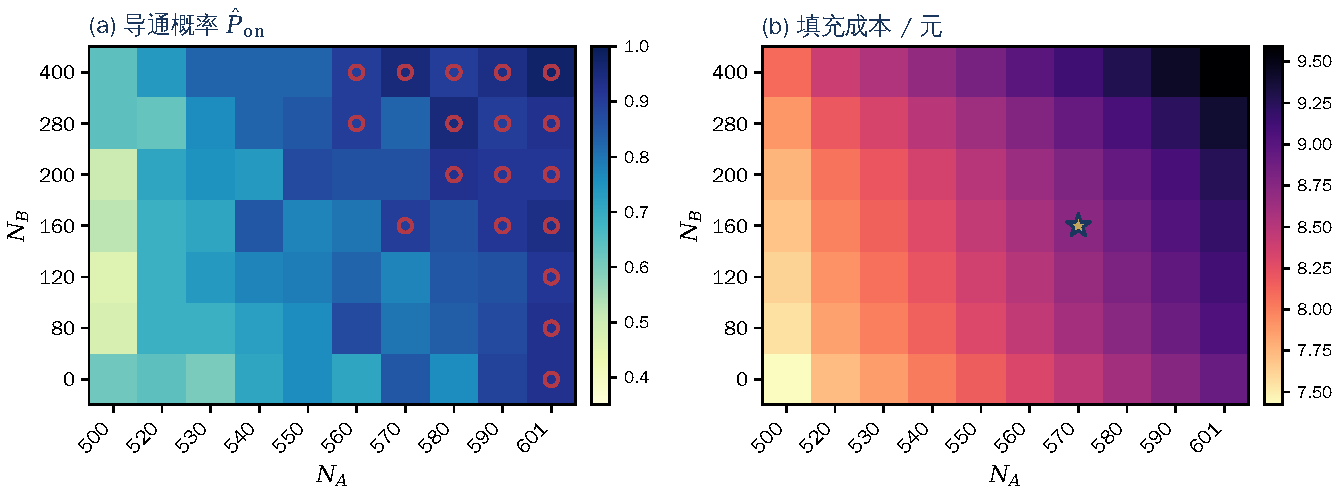
\includegraphics[width=0.96\textwidth]{fig_mixheat}
\caption{混合填充网格的矩阵视图。(a) 导通概率，红圈为 $\hat P\ge 0.90$；(b) 成本，金星为最低成本可行点}
\label{fig:mixheat}
\end{figure}

\begin{table}[H]
\centering
\caption{$P_{\mathrm{on}}\ge 0.90$ 的部分格点（每点 $80$ 次）}
\label{tab:p4}
\begin{tabular}{rrcccc}
\toprule
$N_A$ & $N_B$ & $\varphi_A/\%$ & $\varphi_B/\%$ & $C/$元 & $\hat P_{\mathrm{on}}$ \\
\midrule
570 & 160 & 0.806 & 0.536 & 8.73 & $0.900\pm 0.066$ \\
560 & 280 & 0.792 & 0.938 & 8.78 & $0.900\pm 0.066$ \\
601 & 0   & 0.850 & 0.000 & 8.92 & $0.925\pm 0.058$ \\
580 & 200 & 0.820 & 0.670 & 8.94 & $0.925\pm 0.058$ \\
590 & 160 & 0.834 & 0.536 & 9.03 & $0.912\pm 0.062$ \\
\bottomrule
\end{tabular}
\end{table}

网格内成本最低的可行点为 $(570,160)$，较纯 A 节省 $0.19$ 元（约 $2.2\%$）。该点的 $80$ 次区间半宽达 $6.6$ 个百分点，下界低于 $0.90$。纯 A 点在第 2 问的 $250$ 次试验中 $\hat P=0.908$，证据更充分。把 $N_A$ 降到 $500\sim 540$ 后，即使补上 $400$ 颗球，$\hat P$ 仍多在 $0.63\sim 0.85$，不足以跨过 $90\%$ 阈值，说明球体的接头作用存在，但在本题尺度上不能替代数十根棒的长程跨越。

图\ref{fig:costcurve} 把同一网格改画成``成本--概率''族曲线，每条曲线对应固定的 $N_B$。可以看到：增加球体使曲线向左（更便宜）移动的幅度很小，而向上（更高概率）的抬升在 $N_A\le 540$ 时始终到不了 $0.90$；真正跨线的点都集中在 $N_A\ge 560$ 且成本靠近 $8.7\sim 9.0$ 元的窄带里。这幅图把``球体便宜但不能替代棒''的结论从热图上的定性印象，落实为成本轴上的定量比较。

\begin{figure}[H]
\centering
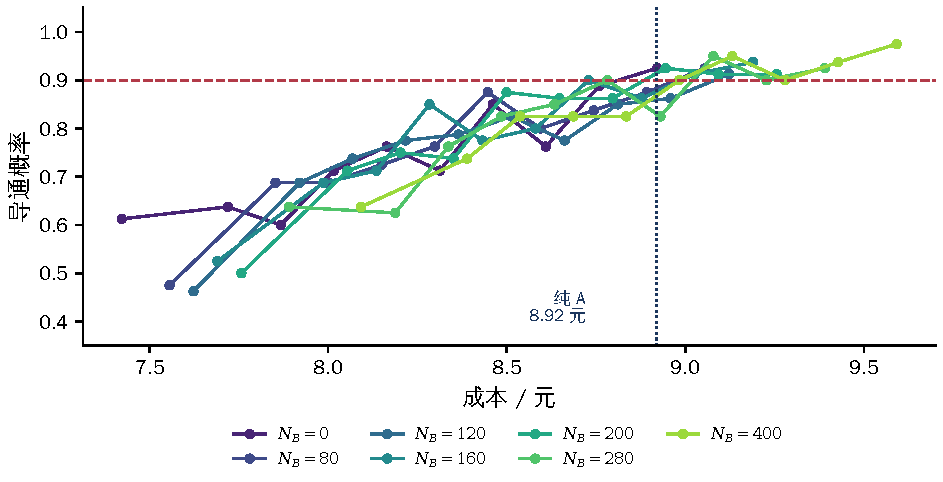
\includegraphics[width=0.78\textwidth]{fig_costcurve}
\caption{固定 $N_B$ 时成本与导通概率的关系。水平虚线为 $90\%$ 约束，竖虚线为纯 A 成本}
\label{fig:costcurve}
\end{figure}

\subsection{推荐方案}

\begin{enumerate}
  \item \textbf{稳健方案（推荐）}：只填充介质 A，$N_A=601$，$\varphi_A=0.85\%$，$N_B=0$，成本 $8.92$ 元。该点由 $250$ 次增量试验支撑，$P_{\mathrm{on}}$ 点估计 $90.8\%$。
  \item \textbf{探索性混合}：$(N_A,N_B)=(570,160)$，即 $\varphi_A=0.81\%$，$\varphi_B=0.54\%$，成本 $8.73$ 元。可作为对接头效应的利用，但若评审口径要求置信下界也超过 $90\%$，则应回到稳健方案。
\end{enumerate}

纯 B 不可行：在 $N_B\le 1200$（成本仅 $2.0$ 元）时导通概率仍为 $0$，与 $\varphi_B^c\approx 29\%$ 的理论判断一致。

\section{综合检验与误差分析}

\subsection{量纲与边界}

全部判定式两端均为长度。电极接触在端点落在 $x=\pm W/2$ 时距离为零，闭区间判定将其计入触极，与附件中大量端点恰好位于边界的数据相容。组 1 两端点均在左边界的三段被正确挂到 $L$，未出现因浮点比较导致的漏挂。

\subsection{有限样本与收敛}

主曲线使用 $M=250$。将样本均分为前后各 $125$ 次，四个体积分数的 $\hat P$ 绝对差不超过 $0.04$，与 $\mathrm{se}$ 同量级。$N_c$ 的最大值 $694$ 比 $N_{\max}=800$ 低百余根，不存在右删失。第 4 问格点的 $M=80$ 使 $P\approx 0.90$ 处的区间半宽约 $0.07$，足以区分``明显可行 / 明显不可行''，不足以精细比较 $2\%$ 量级的成本差，故对混合点只作探索性陈述。

为把样本量选择说清楚，以 $N_A=601$ 处的 $\hat P$ 为对象做 $400$ 次 Bootstrap（图\ref{fig:boot}）。当 $M$ 从 $30$ 增到 $250$，区间半宽由约 $0.12$ 收至约 $0.04$，点估计稳定在 $0.90\sim 0.91$ 并始终位于约束线之上。继续增大 $M$ 对决策不再改变：第 3 问的 $0.85\%$ 不会因为多样本而滑到 $0.84\%$ 或 $0.86\%$。

\begin{figure}[H]
\centering
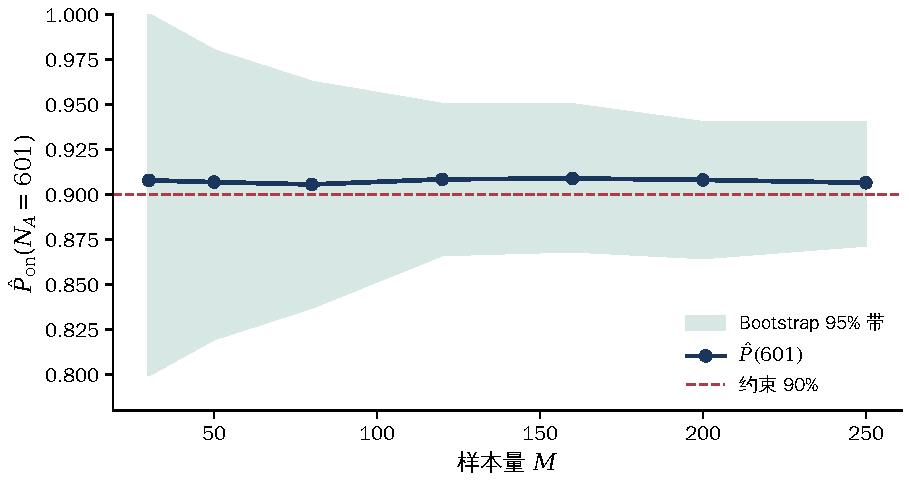
\includegraphics[width=0.78\textwidth]{fig_bootstrap}
\caption{$N_A=601$ 处导通概率估计随样本量的 Bootstrap 收敛。色带为 $95\%$ 分位区间}
\label{fig:boot}
\end{figure}

\subsection{计算复杂度}

单次导通判定的主要代价是段段距离。组 3 有 $n=535$，成对计算 $O(n^2)\approx 1.4\times 10^5$ 次，双精度下毫秒级完成。增量 Monte Carlo 在上限 $N_{\max}=800$ 时，每次投放的距离计算量为
\[
\sum_{k=1}^{N_{\max}}O(k)=O(N_{\max}^2)\approx 3\times 10^5,
\]

250 次合计约 $10^8$ 次线段距离，Numba 编译后可在普通笔记本上数分钟内跑完。混合网格约 $10\times 7=70$ 格、每格 $80$ 次，量级与主曲线相当。空间散列或扫描线可以把渐近阶降到 $O(n\log n)$，对本题规模并无必要。

\subsection{独立算法复核}

并查集与从电极出发的广度优先遍历在第 1 问三组以及第 2 问抽查的 $80$ 个随机构型上给出完全相同的布尔结论。线段距离核用若干平行、正交、端点接触的解析算例核对，最大相对误差低于 $10^{-12}$。

\subsection{敏感性}

隧穿阈值进入排除体积的方式是 $D_{\mathrm{eff}}=2R_A+\delta$。图\ref{fig:sens} 给出 $\varphi_c^{\mathrm{th}}(\delta)$：$\delta$ 在 $1.2\sim 2.4\,\mathrm{nm}$ 内变动时，理论阈值只在 $0.81\%\sim 0.82\%$ 之间微移，因为 $\delta$ 远小于直径。因而第 3 问的 $0.85\%$ 不会因 $\delta$ 的小幅标定误差而跳到相邻的百分号下两位。

\begin{figure}[H]
\centering
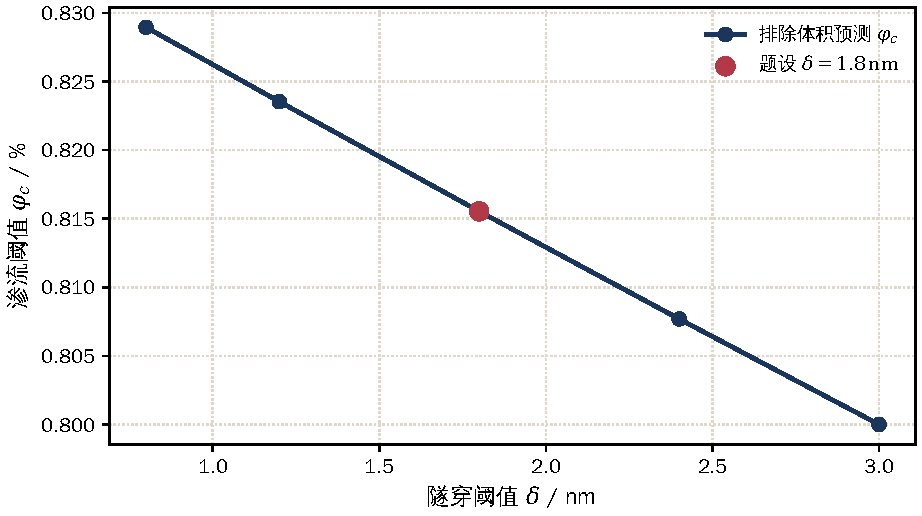
\includegraphics[width=0.80\textwidth]{fig_sens}
\caption{排除体积阈值随隧穿距离的变化。题设 $\delta=1.8\,\mathrm{nm}$ 处曲线极为平缓}
\label{fig:sens}
\end{figure}

完全内含对照系综（图\ref{fig:pphi} 虚线）缺少截断产生的贴面短段，触极更困难，$P_{\mathrm{on}}$ 整体右移，其 $90\%$ 阈值升至约 $1.25\%$。主模型与附件数据形态一致，对照只用于说明：若禁止越界回填，填充量需求会明显上升。两种系综的定性排序（组 1 最稀疏、阈值位于百分位）不变。

把圆柱改成带半球帽的球柱，排除体积只增加 $O(D_{\mathrm{eff}}^3)$ 的端帽项；相对细长主项 $\frac{\pi}{2}L^2 D_{\mathrm{eff}}$，该修正仅约 $0.3\%$，对 $\varphi_c$ 的影响可忽略。

\section{模型评价与推广}

\subsection{优点}

模型把题面的极化规则写成与贯穿相容的闭距离不等式，避免了``先判相交再判隧穿''的分支。公共判定器在四问中原样复用，第 1 问的三组混合结论（一否两是）为后续随机模型提供了非平凡校准。增量 Monte Carlo 用一次投放得到整条概率曲线，使第 2、3 问共享同一组 $N_c$ 样本，统计口径一致。排除体积给出的 $0.82\%$ 与模拟分位相互印证，结论不只依赖``曲线看起来光滑''。

\subsection{局限}

分段独立虽然使问题适定，但把同一母圆柱的两段当成电学上断开的对象，偏保守。真实极化若能沿导体内部跨越截断缝，阈值会下降。有限盒子 $W=2L$ 使结果带有显著有限尺度效应，外推到宏观块体时 $90\%$ 可靠填充量应更接近 $\varphi_c^{\mathrm{th}}$ 而非本盒的 $0.85\%$。第 4 问未对球体作硬核排斥，高 $\varphi_B$ 时名义体积分数会高估真实占有率。混合点的成本优势落在 Monte Carlo 误差带内，不能当成工程上已证实的节省。

\subsection{推广}

更换长径比时，只需用新的 $L,R_A$ 重算 $V_A$ 与 $D_{\mathrm{eff}}$，\eqref{eq:phith} 可作初值，再跑同一套增量程序。若电极改到 $Y$ 或 $Z$ 面，把 \eqref{eq:dplane} 的轴向对调即可。若需要硬核排斥，应在投放阶段加入重叠拒绝，判定核不必改。

若实际工艺允许同一母圆柱在截断后仍保持电学连通（例如导电涂层连续跨过边界回填缝），则应把同母圆柱的子段预先 Union，此时 $P_{\mathrm{on}}(\varphi)$ 会整体左移，第 3 问的可靠填充量将低于 $0.85\%$。本文把该情形作为对照而非主模型，理由是附件把每一行写成独立介质，且题面把提问窗口放在 $0.50\%\sim 1.00\%$——只有分段独立才能让这个窗口具有分辨力。

对宏观块体，有限尺度修正可写成
\[
\varphi_c(W)=\varphi_c^{\infty}+A\,W^{-1/\nu},
\]

其中三维连续渗流 $\nu\approx 0.88$。本题只有一个盒子尺寸 $W=2L$，无法单独拟合 $A$ 与 $\nu$，但 $\varphi_c(W)=0.85\%$ 高于 $\varphi_c^{\mathrm{th}}=0.82\%$ 的方向与该式一致。工程外推时应取接近 $0.82\%$ 的值，并另做更大盒子的核算。

\section{主要结论}

\begin{enumerate}
  \item 组 1 不导通，组 2 导通，组 3 导通。组 1 左右极簇之间不存在满足 $1.8\,\mathrm{nm}$ 阈值的桥。
  \item 体积分数 $0.50\%$、$0.60\%$、$0.70\%$、$1.00\%$ 的导通概率分别为 $10.4\%$、$22.8\%$、$52.0\%$ 与 $100\%$。
  \item $P_{\mathrm{on}}\ge 90\%$ 的最低填充量为 $0.85\%$（$601$ 根介质 A）。排除体积理论值 $0.82\%$ 与之接近。
  \item 稳健最低成本方案为只填充 $601$ 根介质 A，成本 $8.92$ 元；混合点 $(570,160)$ 的标称成本 $8.73$ 元，节省有限且统计证据较弱。
\end{enumerate}

\begin{thebibliography}{99}
\bibitem{balberg1984}
I.~Balberg, C.~H.~Anderson, S.~Alexander, N.~Wagner.
Excluded volume and its relation to the onset of percolation.
\textit{Physical Review B}, 1984, 30(7): 3933--3943.

\bibitem{bug1985}
A.~L.~R.~Bug, S.~A.~Safran, I.~Webman.
Continuum percolation of rods.
\textit{Physical Review Letters}, 1985, 54(13): 1412--1415.

\bibitem{celzard1996}
A.~Celzard, E.~McRae, C.~Deleuze, M.~Dufort, G.~Furdin, J.~F.~Mar\^{e}ch\'{e}.
Critical concentration in percolating systems containing a high-aspect-ratio filler.
\textit{Physical Review B}, 1996, 53(10): 6209--6214.

\bibitem{mutiso2012}
R.~M.~Mutiso, M.~C.~Sherrott, J.~Li, K.~I.~Winey.
Simulations and critical analysis of continuum percolation of rodlike particles.
\textit{Physical Review E}, 2012, 86: 041815.

\bibitem{otten2009}
R.~H.~J.~Otten, P.~van der Schoot.
Continuum percolation of polydisperse nanofillers.
\textit{Physical Review Letters}, 2009, 103: 225704.

\bibitem{newman2001}
M.~E.~J.~Newman, R.~M.~Ziff.
Fast Monte Carlo algorithm for site or bond percolation.
\textit{Physical Review E}, 2001, 64: 016706.

\bibitem{tarjan1975}
R.~E.~Tarjan.
Efficiency of a good but not linear set union algorithm.
\textit{Journal of the ACM}, 1975, 22(2): 215--225.

\bibitem{ericson2004}
C.~Ericson.
\textit{Real-Time Collision Detection}.
Morgan Kaufmann, 2004.

\bibitem{stauffer1994}
D.~Stauffer, A.~Aharony.
\textit{Introduction to Percolation Theory}.
2nd ed. Taylor \& Francis, 1994.

\bibitem{winey2007}
K.~I.~Winey, T.~Kashiwagi, M.~Mu.
Improving electrical conductivity and thermal properties of polymers by the addition of carbon nanotubes as fillers.
\textit{MRS Bulletin}, 2007, 32(4): 348--353.
\end{thebibliography}

\appendix
\section{支撑材料文件列表}

\begin{center}
\small
\begin{tabularx}{\textwidth}{lXl}
\toprule
文件 & 用途 & 依赖 \\
\midrule
\texttt{src/simulate.py} & 几何核、并查集、第 1 问与内含系综 & NumPy, Numba \\
\texttt{src/wrap\_mc.py} & 截断分段增量 Monte Carlo、混合填充 & simulate.py \\
\texttt{src/make\_figures.py} & 正文全部图件 & Matplotlib \\
\texttt{src/geom.py} & 线段距离的可读参考实现 & NumPy \\
\texttt{results/problem1.json} & 第 1 问统计 & --- \\
\texttt{results/problem23\_wrap.json} & 第 2、3 问主结果 & --- \\
\texttt{results/crit\_wrap.npy} & 250 个 $N_c$ 样本 & --- \\
\texttt{results/problem4\_stage2.json} & 第 4 问网格 & --- \\
\texttt{attachments/附件.xlsx} & 题目原始坐标 & --- \\
\bottomrule
\end{tabularx}
\end{center}

运行顺序：先运行 \texttt{simulate.py} 完成第 1 问，再运行 \texttt{wrap\_mc.py} 生成生存曲线，最后运行 \texttt{make\_figures.py} 出图。随机种子见各脚本。

\section{核心算法代码}

第 1 问判定与增量临界个数的核心片段如下。完整可运行程序见 \texttt{src/} 目录。

\begin{lstlisting}[language=Python,caption={并查集与圆柱段导通判定（节选）}]
class UF:
    def __init__(self, n):
        self.p = list(range(n)); self.r = [0]*n
    def find(self, x):
        while self.p[x] != x:
            self.p[x] = self.p[self.p[x]]; x = self.p[x]
        return x
    def union(self, a, b):
        ra, rb = self.find(a), self.find(b)
        if ra == rb: return
        if self.r[ra] < self.r[rb]: ra, rb = rb, ra
        self.p[rb] = ra
        if self.r[ra] == self.r[rb]: self.r[ra] += 1

# A-A: d_seg <= 2*R_A + delta = 61.8 nm
# A-electrode: d_plane <= R_A + delta = 31.8 nm
def is_percolating(P, Q):
    n = len(P); LEFT, RIGHT = n, n+1
    uf = UF(n+2)
    for i in range(n):
        if plane_dist(P[i], Q[i], -5000) <= 31.8: uf.union(i, LEFT)
        if plane_dist(P[i], Q[i], +5000) <= 31.8: uf.union(i, RIGHT)
    for i in range(n):
        for j in range(i+1, n):
            if seg_dist(P[i], Q[i], P[j], Q[j]) <= 61.8:
                uf.union(i, j)
    return uf.find(LEFT) == uf.find(RIGHT)
\end{lstlisting}

\begin{lstlisting}[language=Python,caption={体积分数与个数换算}]
import math
W, L, RA = 10000.0, 5000.0, 30.0
VA = math.pi * RA**2 * L          # 1.4137e7 nm^3
V  = W**3                         # 1e12 nm^3
def N_from_phi(phi):
    return int(round(phi * V / VA))
# 0.50%, 0.60%, 0.70%, 1.00% -> 354, 424, 495, 707
\end{lstlisting}

\section{补充数值表}

\begin{table}[H]
\centering
\caption{$N_c$ 的分位（截断分段系综，$M=250$，$N_{\max}=800$）}
\begin{tabular}{cccccc}
\toprule
最小 & $10\%$ & 中位 & 均值 & $90\%$ & 最大 \\
\midrule
210 & 347 & 492 & 482.7 & 598 & 694 \\
\bottomrule
\end{tabular}
\end{table}

\begin{table}[H]
\centering
\caption{百分号下两位网格上 $\hat P_{\mathrm{on}}$ 在阈值附近的取值}
\begin{tabular}{cccc}
\toprule
$\varphi_A/\%$ & $N_A$ & $\hat P_{\mathrm{on}}$ & 是否 $\ge 0.90$ \\
\midrule
0.80 & 566 & 0.848 & 否 \\
0.82 & 580 & 0.868 & 否 \\
0.83 & 587 & 0.880 & 否 \\
0.84 & 594 & 0.896 & 否 \\
0.85 & 601 & 0.908 & 是 \\
0.86 & 608 & 0.916 & 是 \\
0.90 & 637 & 0.956 & 是 \\
1.00 & 707 & 1.000 & 是 \\
\bottomrule
\end{tabular}
\end{table}

\end{document}
